\chapter{Question 1}
\label{question-1}
\section{Question}

Write a program that extracts 10000 tweets with links from Twitter.

\begin{itemize}
\item Save the tweet URIs, and the mapping to the link(s) each tweet contains.
\item For each t.co link, use ``curl -I -L'' to record the HTTP headers all the way to a terminal HTTP status (i.e. chase down all the redirects)
\item How many unique final URI's? How many duplicate URI's?
\item Build a histogram of how many redirects (every URI will have at least 1)
\item Build a histogram of HTTP status codes encountered (you’ll have at least 20000: 10000 301s, and 10000+ more)
\end{itemize}

\section{Solution}
For solving the above problem I have used Python as the programming language. Following are the steps I've taken to solve the given problem:
\begin{itemize}
\item I first registered a twitter application to generate the consumer key and consumer secret key for using the Twitter API.
\item The key's generated in the above step are used for authenticating the application for requesting the tweets.
\item I encountered multiple packages while researching for packages for fetching tweet data and decided upon TwitterSearch package.
\item I was facing an issue with the TwitterSearch package where I was receiving limited results. In-spite of making modifications to the keyword for search I wasn't able to exceed more than 800 results.
\item I eventually moved to tweepy package with which I was receiving approximately 2000 results and it would stop again. Along with the keyword argument I also passed another argument `since = 2014' to the API search as the tweets fetched would stop at a certain date. This additional argument solved my problem. I was able to retrieve more than 10000 tweets.
\item From the tweet data received from the API, I fetched the tweet identifier, created date, user identifier, tweet text and of course the URI.
\item The above mentioned data was processed to json format and written to a file `output.txt'.
\item For retrieving the final URI, history of status code's encountered, I found requests package to be the most powerful and appropriate for use in my context.
\item I used the requests package in `requestStatus.py' for fetching the above mentioned information and output this information to `status.txt' file.
\item Now with the raw information available, I processed the data further based on the requirement as specified in the question.
\item Based on the tweet data, I found that the number of unique URI's that were encountered were 6431, duplicate links were 3999. The total number of greater than 10000 as some tweets had more than one URI. This information was calculated using script `getUniqueURI.py' and the result was stored in `unique.txt'.
\item Also, I calculated the number of re-directs for each URI using the script `getURIRedirect.py' and the result was stored in 'uriRedirect.txt'. This information was processed through R for generating a histogram as shown in the figure below.\\*
	\begin{minipage}{\linewidth}
		\centering
		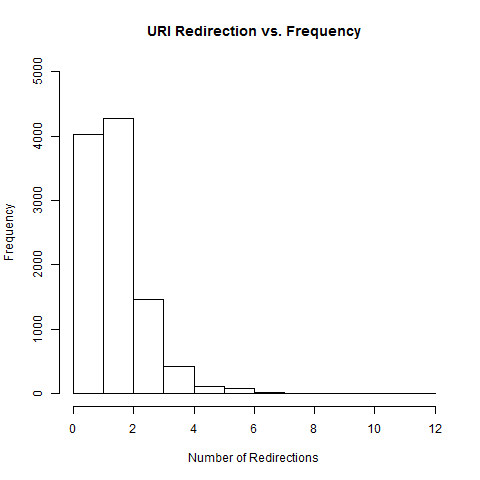
\includegraphics[scale=0.55]{figures/uriRedirect.png}
		\captionof{figure}{URI Redirection vs. Frequency}
		\label{uriRedirect}
	\end{minipage}
\item The raw information from status.txt was also used to calculate the frequency of the status codes encountered for these URI's and the figure below represents the histogram for this data.\\*
	\begin{minipage}{\linewidth}
		\centering
		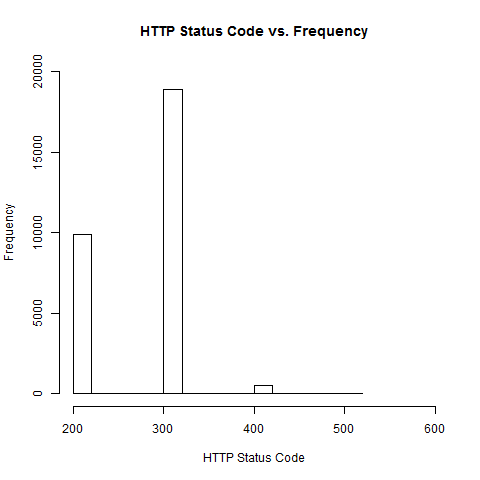
\includegraphics[scale=0.55]{figures/statusCode.png}
		\captionof{figure}{HTTP Status Code vs. Frequency}
		\label{statusCode}
	\end{minipage}	
\end{itemize}

\newpage
\section{Code Listing}
\lstinputlisting[language=Python,breaklines = true,frame=single,caption={Python program for retrieving tweets.},label=lst:q1-1,captionpos=b,numbers=left,showspaces=false,showstringspaces=false,basicstyle=\footnotesize]{pythonFiles/getTweets.py}
\newpage
\lstinputlisting[language=Python,breaklines = true,frame=single,caption={Python program to request the header information for each URI.},label=lst:q1-2,captionpos=b,numbers=left,showspaces=false,showstringspaces=false,basicstyle=\footnotesize]{pythonFiles/requestStatus.py}
\newpage
\lstinputlisting[language=Python,breaklines = true,frame=single,caption={Python program for retrieving the number of unique, duplicate URI's.},label=lst:q1-3,captionpos=b,numbers=left,showspaces=false,showstringspaces=false,basicstyle=\footnotesize]{pythonFiles/getUniqueURI.py}
\newpage
\lstinputlisting[language=Python,breaklines = true,frame=single,caption={Python program for calculating the number of redirects for each URI.},label=lst:q1-4,captionpos=b,numbers=left,showspaces=false,showstringspaces=false,basicstyle=\footnotesize]{pythonFiles/getURIRedirect.py}
\newpage
\lstinputlisting[language=Python,breaklines = true,frame=single,caption={Python program for retrieving the different status codes encountered by each URI.},label=lst:q1-5,captionpos=b,numbers=left,showspaces=false,showstringspaces=false,basicstyle=\footnotesize]{pythonFiles/getStatusCodeFrequency.py}
\newpage
\lstinputlisting[language=R,breaklines = true,frame=single,caption={R program for generating the histogram for URI Redirection vs. Frequency}, label=lst:q1R1,captionpos=b,numbers=left,showspaces=false,showstringspaces=false,basicstyle=\footnotesize]{rFiles/uriRedirect.R}
\lstinputlisting[language=R,breaklines = true,frame=single,caption={R program for generating the histogram for HTTP Status Code vs. Frequency}, label=lst:q1R2,captionpos=b,numbers=left,showspaces=false,showstringspaces=false,basicstyle=\footnotesize]{rFiles/statusCode.R}